%**************************************************************************************************************************
%******************************************************  PREAMBLE  **********************************************************
%**************************************************************************************************************************

\documentclass[10pt]{beamer} %handout,ignorenonframetext
% \setbeameroption{show notes}
% Take out handout option in order to have iterative

%%%%%%%%%%%% Tema 
%---------------------------------
\mode<presentation>{\usetheme{Malmoe}}
\usecolortheme{lily}%{lily}{orchid}

%%%% Footline
% \newcommand*\oldmacro{}%
% \let\oldmacro\insertshorttitle%
% \renewcommand*\insertshorttitle{%
%   \oldmacro\hfill%
%   \insertframenumber\,/\,\inserttotalframenumber}
% \setbeamertemplate{footline}[frame number]

%%%% Headline
%\setbeamertemplate{headline}
%{%
%  \leavevmode%
%  \begin{beamercolorbox}[wd=.5\paperwidth,ht=3.5ex,dp=2.5ex]{section in head/foot}%
%    \hbox to .5\paperwidth{\hfil\insertsectionhead\hfil}
%  \end{beamercolorbox}%
%  \begin{beamercolorbox}[wd=.5\paperwidth,ht=3.5ex,dp=2.5ex]{subsection in head/foot}%
%    \hbox to .5\paperwidth{\hfil\insertsubsectionhead\hfil}
%  \end{beamercolorbox}%
% %}
% Set different sizes in itemize
\setbeamerfont*{itemize/enumerate body}{size=\small}
\setbeamerfont*{itemize/enumerate subbody}{size= \footnotesize}
\setbeamerfont*{itemize/enumerate subsubbody}{size = \footnotesize}

% replaces beamer foot with simple page number
\setbeamertemplate{navigation symbols}{}
\newcommand*\oldmacro{}%
\let\oldmacro\insertshorttitle%
\renewcommand*\insertshorttitle{%
  \hyperlinksectionstart{\secname}\hfill%
  \insertframenumber\,/\,\inserttotalframenumber}
% \setbeamertemplate{footline}{
%   \raisebox{10pt}{\makebox[\paperwidth]{\hfill\makebox[20pt]{\color{gray}\scriptsize\insertpagenumber}}}}


%%%% Justifica o texto dos slides -------------------------------
\usepackage{ragged2e}
% \justifying

%%%% Cores
\usepackage{color}
\setbeamercolor{alerted text}{fg=blue}

%%%% Lista dos Slides
%\usepackage{listliketab}
% Bibliografia
\usepackage{tabu,booktabs , multicol, multirow}


%%%% Pacote Matemática
\usefonttheme[onlymath]{serif}
\usepackage{amsmath, amssymb, amsthm,amsfonts,mathrsfs, bbm}
\usepackage{enumerate,comment}
\DeclareMathOperator*{\Max}{Max}
\DeclareMathOperator*{\Min}{Min}
\DeclareMathOperator*{\argmax}{argmax}


%%%% Figures
\usepackage{graphicx,tabu,float,subfig, epstopdf}%,showframe}
\usepackage[font={normalsize,sc},position=top]{caption}
\usepackage{transparent}

%%%% Environment
\theoremstyle{plain}
\newtheorem{thm}{Theorem}[section]
\newtheorem{lem}[thm]{Lemma}
\newtheorem{prop}[thm]{Proposition}
\newtheorem*{cor}{Corollary}

\theoremstyle{definition}
\newtheorem{defn}{Definition}[section]
\newtheorem{conj}{Conjecture}[section]
\newtheorem{exmp}{Example}[section]

\theoremstyle{remark}
\newtheorem*{rem}{Remark}

%%%% Write code
% \usepackage{minted}
% \newminted{julia}{fontsize=\scriptsize, 
%            mathescape,
%            linenos,
%            numbersep=8pt,
%            gobble=4,
%            frame=lines,
%            framesep=3mm} 

\usepackage{tikz}
\usetikzlibrary{mindmap}                    

%%%% Title
\title{ Heterogeneous Agent Models in Continuous Time \sc }
\subtitle{ HANK }
\author{ Felipe Alves }
\institute[NYU]{NYU}
% \date{}

%**************************************************************************************************************************
%******************************************************  INÍCIO  **********************************************************
%**************************************************************************************************************************
\begin{document}

%%%%%%%%%%%%%%%%%%%%%%%%%%%%%%%%%%%%%%%%%%%%%%%%%%%%%%%%%%%%%%%%%%%%%%%%
%            (1) 
%%%%%%%%%%%%%%%%%%%%%%%%%%%%%%%%%%%%%%%%%%%%%%%%%%%%%%%%%%%%%%%%%%%%%%%%
\begin{frame}
   \titlepage
\end{frame}

%- - - -- - - -- - - -- - - -- - - -- - - -- - - -- - - -- - - -- - - -- 
%       (5) 
%- - - -- - - -- - - -- - - -- - - -- - - -- - - -- - - -- - - -- - - -- 
% \begin{frame}{\emph{Outline}}
%   \tableofcontents
% \end{frame}

%**************************************************************************************************************************
% --------------------------------------------- INTRODUCTION                                                 
%**************************************************************************************************************************
\section{Introduction}

%%%%%%%%%%%%%%%%%%%%%%%%%%%%%%%%%%%%%%%%%%%%%%%%%%%%%%%%%%%%%%%%%%%%%%%%
%                (2)
%%%%%%%%%%%%%%%%%%%%%%%%%%%%%%%%%%%%%%%%%%%%%%%%%%%%%%%%%%%%%%%%%%%%%%%%
\begin{frame}{Outline}{}  \setbeamercovered{transparent}
%  -  -  -  -  -  -  -  -  -  -  -  -  -  -  -  -  -  -  -  -  -  -  -  
\begin{itemize}
% \justifying
    
    \item Heterogeneous Agent Models in Continuous Time 
    \begin{itemize}
        \item Achdou et. al (2014), Moll's website
    \end{itemize} \medskip

    \item solving model = solving PDEs

    \begin{itemize}
        \item Hamilton-Jacobi-Bellman equation for individual choices \smallskip
        \item Kolmogorov Forward equation for evolution of distribution 
    \end{itemize} \medskip

    \item \textbf{Project}: HANK model 

    \begin{itemize}
        \item Household Problem 
    \end{itemize}
\end{itemize}
% ______________________________________________________________________
%  -  -  -  -  -  -  -  -  -  -  -  -  -  -  -  -  -  -  -  -  -  -  -  
\end{frame}

%%%%%%%%%%%%%%%%%%%%%%%%%%%%%%%%%%%%%%%%%%%%%%%%%%%%%%%%%%%%%%%%%%%%%%%%
%                (2)
%%%%%%%%%%%%%%%%%%%%%%%%%%%%%%%%%%%%%%%%%%%%%%%%%%%%%%%%%%%%%%%%%%%%%%%%
\begin{frame}{Textbook Heterog Agent Model}{}  \setbeamercovered{transparent}
%  -  -  -  -  -  -  -  -  -  -  -  -  -  -  -  -  -  -  -  -  -  -  -  
\begin{align*}
    \max_{ c_t } \quad & \mathbb{E}_0 \int_{0}^{\infty} e^{-\rho t} u( c_t) d_t & \\ \ \\
%%%
\text{S.t } \quad   & \dot{a}_t = y_t  + r_t a_t - c_t & \\ \ \\
              & y_t : \text{ Poisson with intensities $\lambda_1, \lambda_2$ } &         \\ 
              & a_t \ge \underbar{a} &
\end{align*}

% ______________________________________________________________________
%  -  -  -  -  -  -  -  -  -  -  -  -  -  -  -  -  -  -  -  -  -  -  -  
\end{frame}



%%%%%%%%%%%%%%%%%%%%%%%%%%%%%%%%%%%%%%%%%%%%%%%%%%%%%%%%%%%%%%%%%%%%%%%%
%            (2) 
%%%%%%%%%%%%%%%%%%%%%%%%%%%%%%%%%%%%%%%%%%%%%%%%%%%%%%%%%%%%%%%%%%%%%%%%
\begin{frame}{Textbook Heterog Agent Model}{} 
%  -  -  -  -  -  -  -  -  -  -  -  -  -  -  -  -  -  -  -  -  -  -  -  -  -  -  -  -  -  -  -  -  -  -  -  -  -  
\begin{itemize}
    \item The value function of the optimal control problem satisfies the HJB equation 
    \begin{equation*}
        \rho v_i( a )  = \max_c\ u(c) +v_i'(a) \Big[ y_i + ra - c \Big] + \lambda_i \Big(v_j( a ) - v_i( a) \Big) 
    \end{equation*} \medskip

    \item Let $G_i(a,t) \equiv P( a_t \le a, y_t = y_i )$. Then
    \begin{equation*}
        \partial_t G_i( a,t ) = -s_i( a,t ) \partial_a G_i( a,t ) - \lambda_i G_i( a,t ) + \lambda_j G_j( a,t )
    \end{equation*}
    while differentiating w.r.t. $a$
    \begin{equation*}
        \partial_t g_i(a,t) = - \frac{d}{da}\big[  s_i( a,t ) g_i( a,t ) \big] - \lambda_i g_i( a,t ) + \lambda_j g_j( a,t )
    \end{equation*}
    

\end{itemize}
%  -  -  -  -  -  -  -  -  -  -  -  -  -  -  -  -  -  -  -  -  -  -  -  -  -  -  -  -  -  -  -  -  -  -  -  -  -  
\end{frame}
%%%%%%%%%%%%%%%%%%%%%%%%%%%%%%%%%%%%%%%%%%%%%%%%%%%%%%%%%%%%%%%%%%%%%%%%
%                (2)
%%%%%%%%%%%%%%%%%%%%%%%%%%%%%%%%%%%%%%%%%%%%%%%%%%%%%%%%%%%%%%%%%%%%%%%%
\begin{frame}{Equilibrium}{}  \setbeamercovered{transparent}
%  -  -  -  -  -  -  -  -  -  -  -  -  -  -  -  -  -  -  -  -  -  -  -  
\begin{align}
    \rho v_i (a) & = \max_c \  u(c) +v_i'(a) \Big[ y_i + ra - c \Big] + \lambda_i \Big(v_j( a ) - v_i( a) \Big) \tag{HJB} \\ 
    \notag \\
    0            & = - \frac{d}{da}\Big[ s_i(a) g_i(a) \Big] - \lambda_i g_i( a ) + \lambda_j g_j( a )  \tag{KF} \\ \
    \notag \\
    0            & = \int a g_1(a) da + \int a g_2( a )da  \tag{equil}
\end{align} \medskip

\alert{Question:} What about state constraint? \medskip

\scriptsize
\emph{state constraint boundary condition: }$v_i'( \underbar{a} ) \ge u'( y_i + r \underbar{a})$

% ______________________________________________________________________
%  -  -  -  -  -  -  -  -  -  -  -  -  -  -  -  -  -  -  -  -  -  -  -  
\end{frame}

%%%%%%%%%%%%%%%%%%%%%%%%%%%%%%%%%%%%%%%%%%%%%%%%%%%%%%%%%%%%%%%%%%%%%%%%
%                (2)
%%%%%%%%%%%%%%%%%%%%%%%%%%%%%%%%%%%%%%%%%%%%%%%%%%%%%%%%%%%%%%%%%%%%%%%%
\begin{frame}{How to solve}{}  \setbeamercovered{transparent}
%  -  -  -  -  -  -  -  -  -  -  -  -  -  -  -  -  -  -  -  -  -  -  -  
\alert{Theoretical background:} Viscosity solutions (??)

\bigskip \bigskip

\alert{Numerical solution\quad  \quad :} Finite Difference methods \medskip
\begin{itemize}
% \justifying
    \item finite difference scheme converges to unique viscosity solution under
    some conditions - \emph{Barles and Souganidis (1991)}

    \begin{enumerate}
        \item Monotonicity \smallskip
        \item Consistency  \smallskip
        \item Stability    \smallskip
    \end{enumerate}
\end{itemize}
% ______________________________________________________________________
%  -  -  -  -  -  -  -  -  -  -  -  -  -  -  -  -  -  -  -  -  -  -  -  
\end{frame}

%%%%%%%%%%%%%%%%%%%%%%%%%%%%%%%%%%%%%%%%%%%%%%%%%%%%%%%%%%%%%%%%%%%%%%%%
%                (2)
%%%%%%%%%%%%%%%%%%%%%%%%%%%%%%%%%%%%%%%%%%%%%%%%%%%%%%%%%%%%%%%%%%%%%%%%
\begin{frame}{Finite Difference Approximation}{HJB equation}  \setbeamercovered{transparent}
%  -  -  -  -  -  -  -  -  -  -  -  -  -  -  -  -  -  -  -  -  -  -  -  
\begin{itemize}
% \justifying
    
    \item Let's approximate $(v_1,v_2 )$ at $J$ discrete points in 
    the space dimension $ a_j$. Putting $ v_{i,j} \equiv v_i( a_j )  $
    \begin{align*}
        \rho v_{i,j} & = u( c_{i,j} ) + v'_{i,j} \Big[  y_i + ra_j - c_{i,j} \Big] + \lambda_i ( v_{-i,j} - v_{i,j} ) \\
        c_{i,j}      & = ( u' )^{-1} ( v'_{i,j} )
    \end{align*}

    \item \alert{PROBLEMS}
    \begin{enumerate}
        \item forward/backward difference approximation $ \rightarrow $ \alert{upwind scheme} \medskip
\begin{equation*}
    \label{eq:1}
    v_{i,j,F}' = \frac{ v_{i,j+1} - v_{i,j} }{ \Delta a }, \qquad v_{i,j,B}' = \frac{ v_{i,j} - v_{i,j-1} }{ \Delta a }
\end{equation*}
        \item How to solve for it? $ \rightarrow $ \alert{explicit $ \times $ implicit method}
    \end{enumerate}

\end{itemize}
% ______________________________________________________________________
%  -  -  -  -  -  -  -  -  -  -  -  -  -  -  -  -  -  -  -  -  -  -  -  
\end{frame}

%%%%%%%%%%%%%%%%%%%%%%%%%%%%%%%%%%%%%%%%%%%%%%%%%%%%%%%%%%%%%%%%%%%%%%%%
%                (2)
%%%%%%%%%%%%%%%%%%%%%%%%%%%%%%%%%%%%%%%%%%%%%%%%%%%%%%%%%%%%%%%%%%%%%%%%
\begin{frame}{Finite Difference Approximation}{HJB equation}  \setbeamercovered{transparent}
%  -  -  -  -  -  -  -  -  -  -  -  -  -  -  -  -  -  -  -  -  -  -  -  

\only<1>{
Let's forget about idisyncratic income shock for a while \bigskip

\alert{\sc Upwind}
\begin{equation*}
    \rho v_{j} = u( c_{j} ) + ( v_{j,B} )' \Big[ y + ra_j - c_{j} \Big]^{-} + ( v_{j,F} )' \Big[ y + ra_j - c_{j} \Big]^{+} 
\end{equation*} \smallskip
}

\only<2>{
\alert{\sc Implicit Method}
\begin{align*}
    & \frac{ v^{n+1}_{j} - v^n_j}{\Delta} + \rho v_{j}^{n+1} =  u( c_{j}^n ) + 
    \frac{ v^{n+1}_j - v^{n+1}_{j-1} }{\Delta a} \Big( s^n_{j,B} \Big)^{-} +
    \frac{ v^{n+1}_{j+1} - v^{n+1}_j }{\Delta a} \Big( s^n_{j,F} \Big)^{+} \\
    & c^n_{j,B} = ( u' )^{-1}( v_{j,B}^n' ), \ c^n_{j,F} = ( u' )^{-1}( v_{j,F}^n' ),  
\end{align*} \smallskip

On a matrix form
\begin{equation*}
    \label{eq:2}
    \frac{1}{\Delta} ( v^{n+1} -v^n ) + \rho v^{n+1} = u^n + \mathbf{A}^n v^{n+1}
\end{equation*}

$  \mathbf{A}^n $: Poison transition matrix / intensity matrix
}
% ______________________________________________________________________
\note{\scriptsize
Summary of Algorithm
\begin{itemize}
% \justifying
    
    \item Compute $ ( v^n_{j} )' $ \smallskip
    
    \item Compute $ c^n $ from $ c^n_{j} = (u')^{-1}\Big[ ( v^n_j )' \Big] $ \smallskip

    \item Find $ v^{n+1} $

\end{itemize}
}
%  -  -  -  -  -  -  -  -  -  -  -  -  -  -  -  -  -  -  -  -  -  -  -  
\end{frame}


%%%%%%%%%%%%%%%%%%%%%%%%%%%%%%%%%%%%%%%%%%%%%%%%%%%%%%%%%%%%%%%%%%%%%%%%
%                (2)
%%%%%%%%%%%%%%%%%%%%%%%%%%%%%%%%%%%%%%%%%%%%%%%%%%%%%%%%%%%%%%%%%%%%%%%%
\begin{frame}{Computational Advantages}{}  \setbeamercovered{transparent}
%  -  -  -  -  -  -  -  -  -  -  -  -  -  -  -  -  -  -  -  -  -  -  -  
\begin{itemize}
% \justifying
    
    \item \textbf{Maximization Problem}
    \only<1>{
    \begin{equation*}
        c^{-\gamma} =  \partial_a v( a, y ) \qquad c^{-\gamma} \ge \beta \int \partial_a v( a', y'  ) dF( y'|y )
    \end{equation*}
    \begin{itemize}
        \item  solve by hand \smallskip
        \item tomorrow is today - no need to compute integrals \smallskip
        \item foc always hold with equality - state constraint boundary condition
    \end{itemize}
    } \bigskip \bigskip

    \item<2-> \textbf{Sparsity}
    \only<2>{
    \begin{itemize}
        \item solving HJB, KFE = inverting matrix \smallskip
        \item but matrices are \emph{sparse} ( Why? )
    \end{itemize}    
    } \bigskip \bigskip

    \item<3-> \textbf{Two birds with one Stone}
    \only<3>{
    \begin{itemize}
        \item tight link between solving HJB equation and KF equation for distribution \smallskip
        \item matrix in discrete KF is \alert{transpose} of $\mathbf{A}$ in HJB
    \end{itemize}    
    }

\end{itemize}
% ______________________________________________________________________
%  -  -  -  -  -  -  -  -  -  -  -  -  -  -  -  -  -  -  -  -  -  -  -  
\end{frame}

%%%%%%%%%%%%%%%%%%%%%%%%%%%%%%%%%%%%%%%%%%%%%%%%%%%%%%%%%%%%%%%%%%%%%%%%
%                (2)
%%%%%%%%%%%%%%%%%%%%%%%%%%%%%%%%%%%%%%%%%%%%%%%%%%%%%%%%%%%%%%%%%%%%%%%%
\begin{frame}{Computational Advantages}{}  \setbeamercovered{transparent}
%  -  -  -  -  -  -  -  -  -  -  -  -  -  -  -  -  -  -  -  -  -  -  -  
\begin{itemize}
% \justifying
    
    \item Maximization Problem
    \begin{equation*}
        c^{-\gamma} =  \partial_a v( a, y ) \qquad c^{-\gamma} \ge \beta \int \partial_a v( a', y'  ) dF( y'|y )
    \end{equation*}
    \begin{itemize}
        \item solve by hand \smallskip
        \item tomorrow is today - no need to compute integrals \smallskip
        \item foc always hold with equality
    \end{itemize}
    \bigskip

    \item Sparsity 
    \begin{itemize}
        \item solving HJB, KFE = inverting matrix \smallskip
        \item but matrices are \emph{sparse}      \smallskip
        \item Why?
    \end{itemize}    
    \bigskip

    \item \emph{Two birds with one Stone}
    \begin{itemize}
        \item tight link between solving HJB equation and KF equation for distribution \smallskip
        \item matrix in discrete KF is \alert{transpose} of $\mathbf{A}$ in HJB
    \end{itemize}    
    

\end{itemize}
% ______________________________________________________________________
%  -  -  -  -  -  -  -  -  -  -  -  -  -  -  -  -  -  -  -  -  -  -  -  
\end{frame}

%%%%%%%%%%%%%%%%%%%%%%%%%%%%%%%%%%%%%%%%%%%%%%%%%%%%%%%%%%%%%%%%%%%%%%%%
%                (2)
%%%%%%%%%%%%%%%%%%%%%%%%%%%%%%%%%%%%%%%%%%%%%%%%%%%%%%%%%%%%%%%%%%%%%%%%
\begin{frame}{HANK}{}  \setbeamercovered{transparent}
%  -  -  -  -  -  -  -  -  -  -  -  -  -  -  -  -  -  -  -  -  -  -  -  
\begin{itemize}
% \justifying
    
    \item Framework for quantitative analysis of aggregate shocks and macroeconomic policy \bigskip

    \item Building blocks
    \begin{enumerate}
        \item uninsurable idiosyncratic income risk \medskip
        \item assets with different degrees of liquidity \medskip
        \item nominal price rigidities 
    \end{enumerate} \bigskip

    \item No aggregate shocks \bigskip

    \item \alert{Today}: only the Household Problem

\end{itemize}
% ______________________________________________________________________
%  -  -  -  -  -  -  -  -  -  -  -  -  -  -  -  -  -  -  -  -  -  -  -  
\end{frame}


%%%%%%%%%%%%%%%%%%%%%%%%%%%%%%%%%%%%%%%%%%%%%%%%%%%%%%%%%%%%%%%%%%%%%%%%
%                (2)
%%%%%%%%%%%%%%%%%%%%%%%%%%%%%%%%%%%%%%%%%%%%%%%%%%%%%%%%%%%%%%%%%%%%%%%%
\begin{frame}{Households}{}  
%  -  -  -  -  -  -  -  -  -  -  -  -  -  -  -  -  -  -  -  -  -  -  -  
\begin{flalign*} 
    \max_{ \{ c_t,  {\transparent{0.1}\color{blue} \ell_t, d_t } \}} & 
    \mathbb{E}_0 \int_{0}^{\infty} e^{-\rho t} u( c_t,  {\transparent{0.1}\color{blue}  \ell_t }) d_t & \\ \ \\
%%%
\text{S.t } \quad   &  \dot{b}_t  = z_t  {\transparent{0.1}\color{blue} w_t  \ell_t - } { \transparent{0.1}\color{blue} \tilde{T}_t( w_t z_t \ell_t)}  + r^b_t {\transparent{0.1}\color{blue} ( b_t ) } b_t 
    {\transparent{0.1}\color{blue} - \Big( d_t + \chi( d_t,a_t ) \Big) } - c_t & \\
      & {\transparent{0.1}\color{blue} \dot{a}_t = r^a_t a_t + d_t } &\\
      & z_t : \text{ Markov Process } &\\
      &b_t \ge \underbar{b}, {\transparent{0.1}\color{blue} \quad a_t \ge 0 } &
\end{flalign*}
% ______________________________________________________________________
%  -  -  -  -  -  -  -  -  -  -  -  -  -  -  -  -  -  -  -  -  -  -  -  
\end{frame}

%%%%%%%%%%%%%%%%%%%%%%%%%%%%%%%%%%%%%%%%%%%%%%%%%%%%%%%%%%%%%%%%%%%%%%%%
%                (2)
%%%%%%%%%%%%%%%%%%%%%%%%%%%%%%%%%%%%%%%%%%%%%%%%%%%%%%%%%%%%%%%%%%%%%%%%
\begin{frame}{Households}{}  \setbeamercovered{transparent}
%  -  -  -  -  -  -  -  -  -  -  -  -  -  -  -  -  -  -  -  -  -  -  -  
\begin{flalign*} 
    \max_{ \{ c_t, \ell_t,   {\transparent{0.1}\color{blue}  d_t } \}} & \mathbb{E}_0 \int_{0}^{\infty} e^{-\rho t} u( c_t, \ell_t) d_t & \\ \ \\
%%%
\text{S.t } \quad   &  \dot{b}_t  = z_t  w_t  \ell_t - \tilde{T}_t( w_t z_t \ell_t)  + r^b_t ( b_t ) b_t 
    {\transparent{0.1}\color{blue} - \Big( d_t + \chi( d_t,a_t ) \Big) } - c_t & \\
      & {\transparent{0.1}\color{blue} \dot{a}_t = r^a_t a_t + d_t } &\\
      & z_t : \text{ Markov Process } &\\
      &b_t \ge \underbar{b}, {\transparent{0.1}\color{blue} \quad a_t \ge 0 } &
\end{flalign*}

% \colorbox{yellow}{%
%   \bfseries
%   \color{blue}%
%   Blue and %
%   \transparent{0.6}%
%   transparent blue%
% }
% ______________________________________________________________________
%  -  -  -  -  -  -  -  -  -  -  -  -  -  -  -  -  -  -  -  -  -  -  -  
\end{frame}


%%%%%%%%%%%%%%%%%%%%%%%%%%%%%%%%%%%%%%%%%%%%%%%%%%%%%%%%%%%%%%%%%%%%%%%%
%                (2)
%%%%%%%%%%%%%%%%%%%%%%%%%%%%%%%%%%%%%%%%%%%%%%%%%%%%%%%%%%%%%%%%%%%%%%%%
\begin{frame}{Households}{}  \setbeamercovered{transparent}
%  -  -  -  -  -  -  -  -  -  -  -  -  -  -  -  -  -  -  -  -  -  -  -  

\begin{flalign*}
    \max_{ \{ c_t, \ell_t, d_t\}} & \mathbb{E}_0 \int_{0}^{\infty} e^{-\rho t} u( c_t, \ell_t) d_t & \\ \ \\
%%%
\text{S.t } \quad   & \dot{b}_t = z_t w_t \ell_t - \tilde{T}_t( w_t z_t \ell_t) + r^b_t( b_t ) b_t 
    - \Big( d_t + \chi( d_t,a_t ) \Big) - c_t &         \\
              & \dot{a}_t = r^a_t a_t + d_t &           \\
              & z_t : \text{ Markov Process } &         \\
              & b_t \ge \underbar{b}, \quad a_t \ge 0 &
\end{flalign*} \smallskip
Adjustment Cost:
    $\chi( d, a) = \underbrace{\vphantom{ \left( \frac{d}{a}\right)^2 } \chi_0 \mathbbm{1} {\{d\ne 0 \}}}_{\text{inaction}} 
    \ + \ 
    \underbrace{\frac{\chi_1}{2} \left( \frac{d}{a}\right)^2 a}_{\text{finite depo}}$ \medskip

Partial Equil: $\Big\{ w, \tilde{T}(\cdot), r^b( b ), r^a \Big\}$


% ______________________________________________________________________
%  -  -  -  -  -  -  -  -  -  -  -  -  -  -  -  -  -  -  -  -  -  -  -  
\end{frame}

%%%%%%%%%%%%%%%%%%%%%%%%%%%%%%%%%%%%%%%%%%%%%%%%%%%%%%%%%%%%%%%%%%%%%%%%
%                (2)
%%%%%%%%%%%%%%%%%%%%%%%%%%%%%%%%%%%%%%%%%%%%%%%%%%%%%%%%%%%%%%%%%%%%%%%%
\begin{frame}{Code Structure}{}  \setbeamercovered{transparent}
%  -  -  -  -  -  -  -  -  -  -  -  -  -  -  -  -  -  -  -  -  -  -  -  
\textsc{Important types}
   
\begin{itemize}
    \item \texttt{TwoAssetsProblem} \medskip

    \item \texttt{Solution} \medskip

    \item \texttt{FDSpec} \medskip
    \begin{itemize}
        \item \texttt{GridInfo}
        \item \texttt{Solution}
    \end{itemize} \medskip

    \item \texttt{SteadyState} \medskip

    \item \texttt{Transition}
\end{itemize}
% ______________________________________________________________________
%  -  -  -  -  -  -  -  -  -  -  -  -  -  -  -  -  -  -  -  -  -  -  -  
\end{frame}

%%%%%%%%%%%%%%%%%%%%%%%%%%%%%%%%%%%%%%%%%%%%%%%%%%%%%%%%%%%%%%%%%%%%%%%%
%                (2)
%%%%%%%%%%%%%%%%%%%%%%%%%%%%%%%%%%%%%%%%%%%%%%%%%%%%%%%%%%%%%%%%%%%%%%%%
\begin{frame}{}{}  \setbeamercovered{transparent}
%  -  -  -  -  -  -  -  -  -  -  -  -  -  -  -  -  -  -  -  -  -  -  -  
%- -.- -.- -.- -.- -.- -.- -.- -.- -.- -.- -.- -.- -.- -.- -.- -.-
%%%%%%%%%%%%%%%% FIGURE: Contour plot
%- -.- -.- -.- -.- -.- -.- -.- -.- -.- -.- -.- -.- -.- -.- -.- -.-
\captionsetup{labelformat=empty, indention=0pt}
\begin{figure}[]
    \caption[]{ Contour plot } \vspace{-10pt}
    \centering
    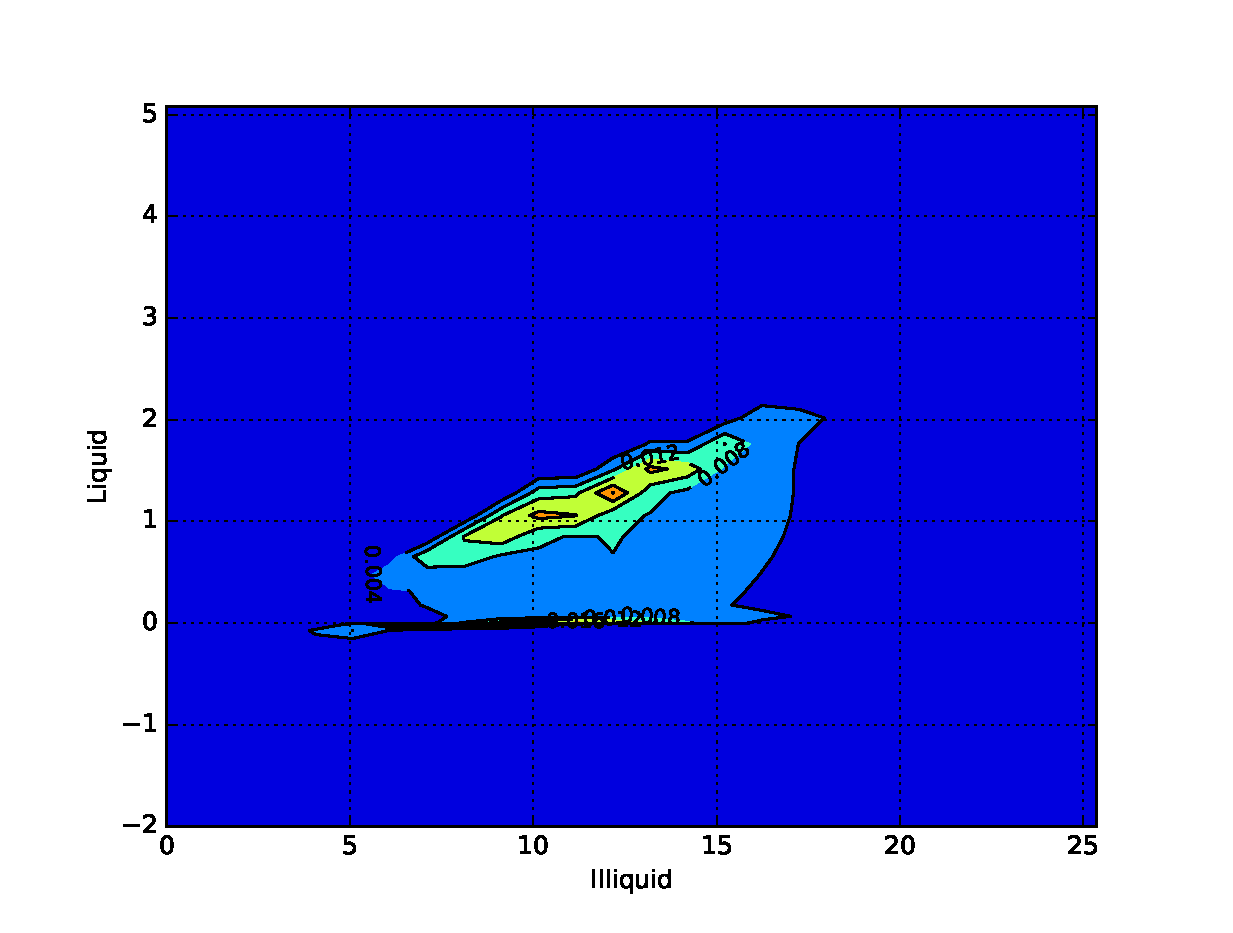
\includegraphics[width=1.0\textwidth]{figure01}
    \label{fig:countor} 
    %%%%%%%%%%%%%%%%
    \captionsetup{font={scriptsize,up},position=below,width=0.8\textwidth}
    \vspace{-0.10cm}
    \caption*{\scriptsize\emph{Note}: }
\end{figure} 

% ______________________________________________________________________
%  -  -  -  -  -  -  -  -  -  -  -  -  -  -  -  -  -  -  -  -  -  -  -  
\end{frame}

%%%%%%%%%%%%%%%%%%%%%%%%%%%%%%%%%%%%%%%%%%%%%%%%%%%%%%%%%%%%%%%%%%%%%%%%
%                (2)
%%%%%%%%%%%%%%%%%%%%%%%%%%%%%%%%%%%%%%%%%%%%%%%%%%%%%%%%%%%%%%%%%%%%%%%%
\begin{frame}{}{}  \setbeamercovered{transparent}
%  -  -  -  -  -  -  -  -  -  -  -  -  -  -  -  -  -  -  -  -  -  -  -  
%- -.- -.- -.- -.- -.- -.- -.- -.- -.- -.- -.- -.- -.- -.- -.- -.-
%%%%%%%%%%%%%%%% FIGURE: Contour plot
%- -.- -.- -.- -.- -.- -.- -.- -.- -.- -.- -.- -.- -.- -.- -.- -.-
\captionsetup{labelformat=empty, indention=0pt}
\begin{figure}[]
    \caption[]{ 3Dplot } \vspace{-10pt}
    \centering
    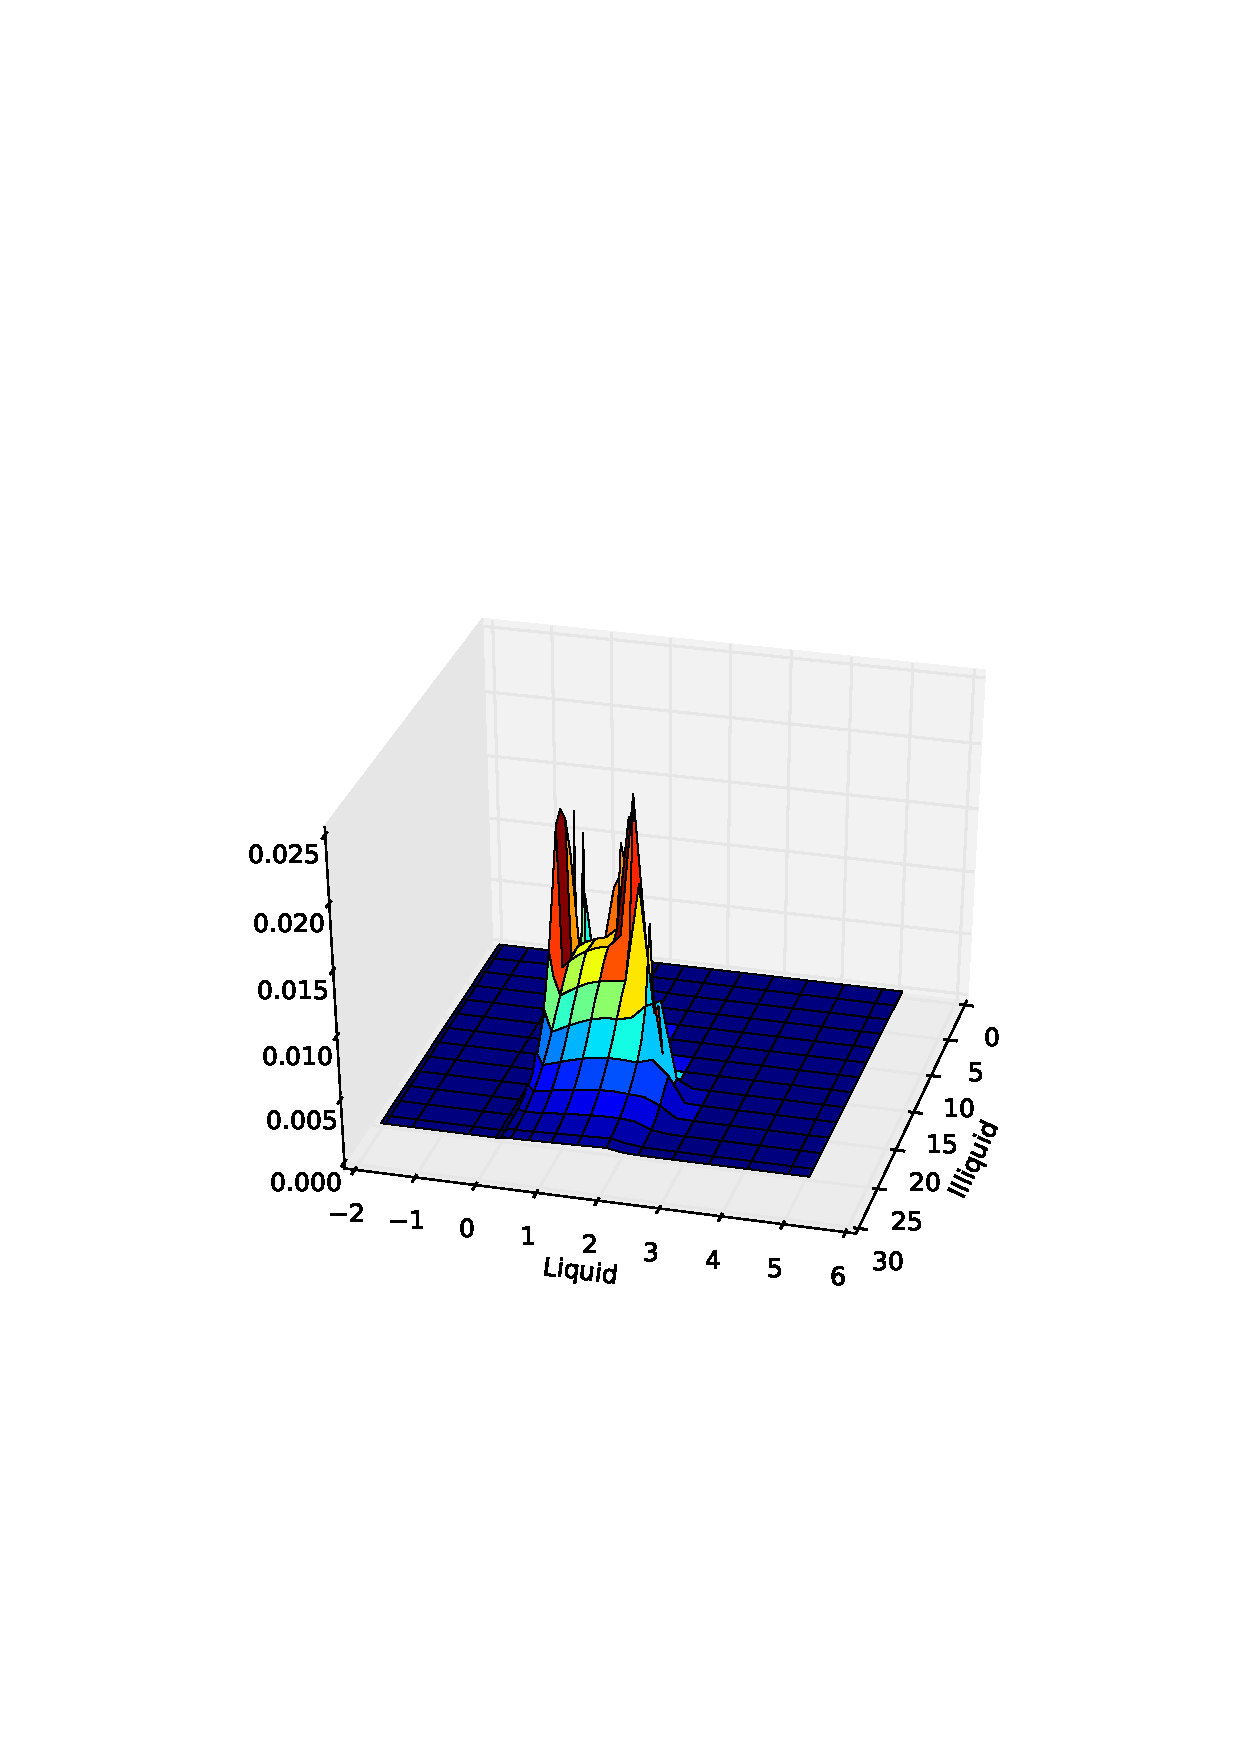
\includegraphics[width=1.0\textwidth]{figure02.png}
    \label{fig:countor} 
    %%%%%%%%%%%%%%%%
    \captionsetup{font={scriptsize,up},position=below,width=0.8\textwidth}
    \vspace{-0.10cm}
    \caption*{\scriptsize\emph{Note}: }
\end{figure} 

% ______________________________________________________________________
%  -  -  -  -  -  -  -  -  -  -  -  -  -  -  -  -  -  -  -  -  -  -  -  
\end{frame}

% \defverbatim[colored]\exampleCode{
% \begin{juliacode}
                
%     type TwoAssetsProb
%     gamma::Float64      # CRRA utility with parameter gamma
%     rho  ::Float64      # discount rate
%     xi   ::Float64      # automatic deposit on illiquid asset
%     sigma::Float64
%     psi  ::Float64

%     rᴬ   ::Float64    # ret on illiquid asset
%     rᴮ   ::Float64    # ret on liq asset
%     wedge::Float64
%     w    ::Float64    # wage rate

%     tau::Float64
%     T::Float64

%     chi0::Float64     # parameters on adjustment cost
%     chi1::Float64
%     end  

% \end{juliacode}
% }

% \begin{frame}
% \frametitle{Code example}
% \exampleCode
% \end{frame}


% %%%%%%%%%%%%%%%%%%%%%%%%%%%%%%%%%%%%%%%%%%%%%%%%%%%%%%%%%%%%%%%%%%%%%%%%
% %            (2) 
% %%%%%%%%%%%%%%%%%%%%%%%%%%%%%%%%%%%%%%%%%%%%%%%%%%%%%%%%%%%%%%%%%%%%%%%%
% \begin{frame}{text}[fragile]
% %  -  -  -  -  -  -  -  -  -  -  -  -  -  -  -  -  -  -  -  -  -  -  -  -  -  -  -  -  -  -  -  -  -  -  -  -  -  
%     \begin{minted}{c} int main() {
%         printf("hello, world");
%         return 0;
%         }
%     \end{minted}
% \end{frame}


%**************************************************************************************************************************
%******************************************************          **********************************************************
%**************************************************************************************************************************

\end{document}